
\section{frog cartoon figures}
\subsection{pepe the frog}
\begin{figure}[h]
\begin{center}

\includegraphics[width=0.4\textwidth]{frog/image/angry.png} 
\caption{when you are debuging your tex file...}
\label{figurezzzz}
\end{center}
\end{figure}
Pepe the Frog is a popular Internet meme. A green anthropomorphic frog with a humanoid body, Pepe originated in a comic by Matt Furie called Boy's Club.It became an Internet meme when its popularity steadily grew across Myspace, Gaia Online and 4chan in 2008. By 2015, it had become one of the most popular memes used on 4chan and Tumblr.Different types of Pepe include "Sad Frog", "Smug Frog", "Angry Pepe", "Feels Frog", and "You will never..." Frog. Since 2014, "Rare Pepes" have been posted on the (sarcastic) "meme market" as if they were trading cards.
\begin{figure}[h]
\begin{center}

\includegraphics[width=0.4\textwidth]{frog/image/frog.jpg} %ajustement de taille
\caption{sad pepe}
\label{figurezzzz}
\end{center}
\end{figure}
\begin{figure}[h]
\begin{center}
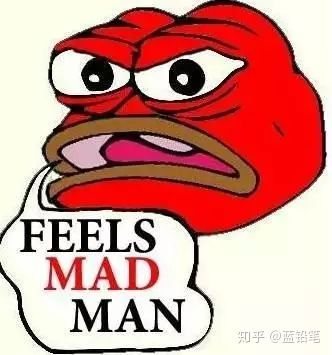
\includegraphics[width=0.5\textwidth]{frog/image/mad.jpg} %ajustement de taille
\caption{mad pepe}
\label{figurezzzz}
\end{center}
\end{figure}
By 2016, the character's image had been appropriated[8] as a symbol of the controversial alt-right movement.[9] The Anti-Defamation League added certain incarnations of Pepe the Frog to their database of hate symbols in 2016, adding that not all Pepe memes are racist.[10] Since then, Pepe's creator has publicly expressed his dismay at Pepe being used as a hate symbol.
Pepe the Frog’s battles are finally over. Cartoonist Matt Furie has officially killed off his most famous creation, which rose from internet meme to white supremacist mascot during the 2016 US election. As reported by Comic Book Resources, Furie published a one-page installment of his “Boy’s Club” series (where Pepe was first introduced in 2005) in celebration of Free Comic Book Day. The strip shows Pepe laid to rest in an open casket while his friends gather round to mourn. One pours out some whisky for the departed frog, splashing it on Pepe’s face. 
\begin{center}
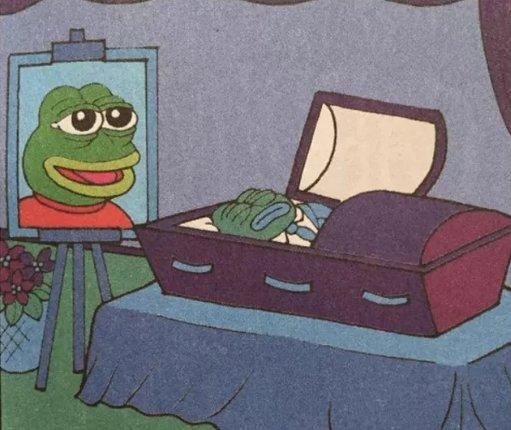
\includegraphics[width=0.4\textwidth]{frog/image/frog2.jpg}
\end{center}
Furie hasn’t spoken about the new cartoon, but its publication seems to bring to an end his quest to rehabilitate Pepe. When the alt-right version of the cartoon became a widespread meme last year, Furie was initially upbeat, saying Pepe’s political affiliation was just “a phase,” and that the cartoon’s “lovable, and charming status will be intact as early as next week.” 

\subsection{travel frog}
A Japanese mobile game about a traveling frog is teaching its fans a philosophical lesson about letting go

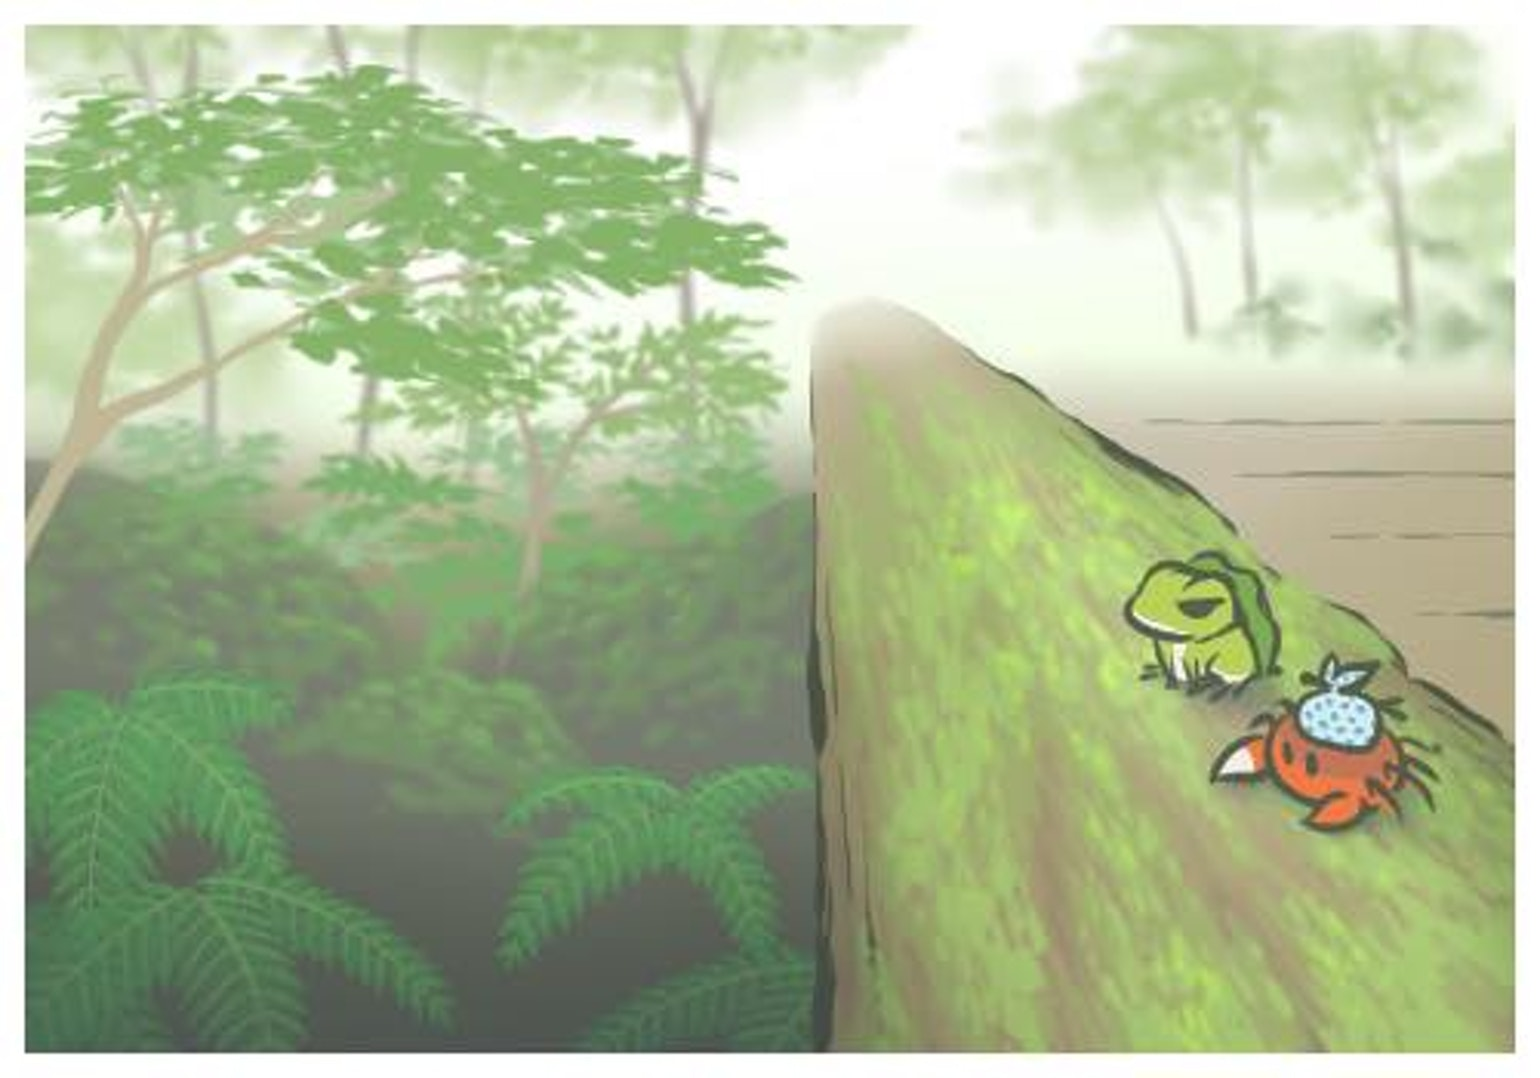
\includegraphics[width=.5\textwidth]{frog/image/voyagefrog.jpg}

Travel Frog, or Tabi Kaeru, has been topping Apple’s App Store across mainland China, Hong Kong and Taiwan since its release two months ago. It’s been downloaded around 4 million times from China’s App Store since December, according to the BBC. Created by Hit-Point, the Japanese company responsible for the popular Kitty Collector (Neko Atsume) in 2014, play involves helping your frog prepare for its solo journey by providing it with food and money—yet the player has no control over when and where the frog goes, or when it will return. The frog communicates with the player with, ironically for a digital game, postcards from his traveling destinations.
\begin{figure}[h]
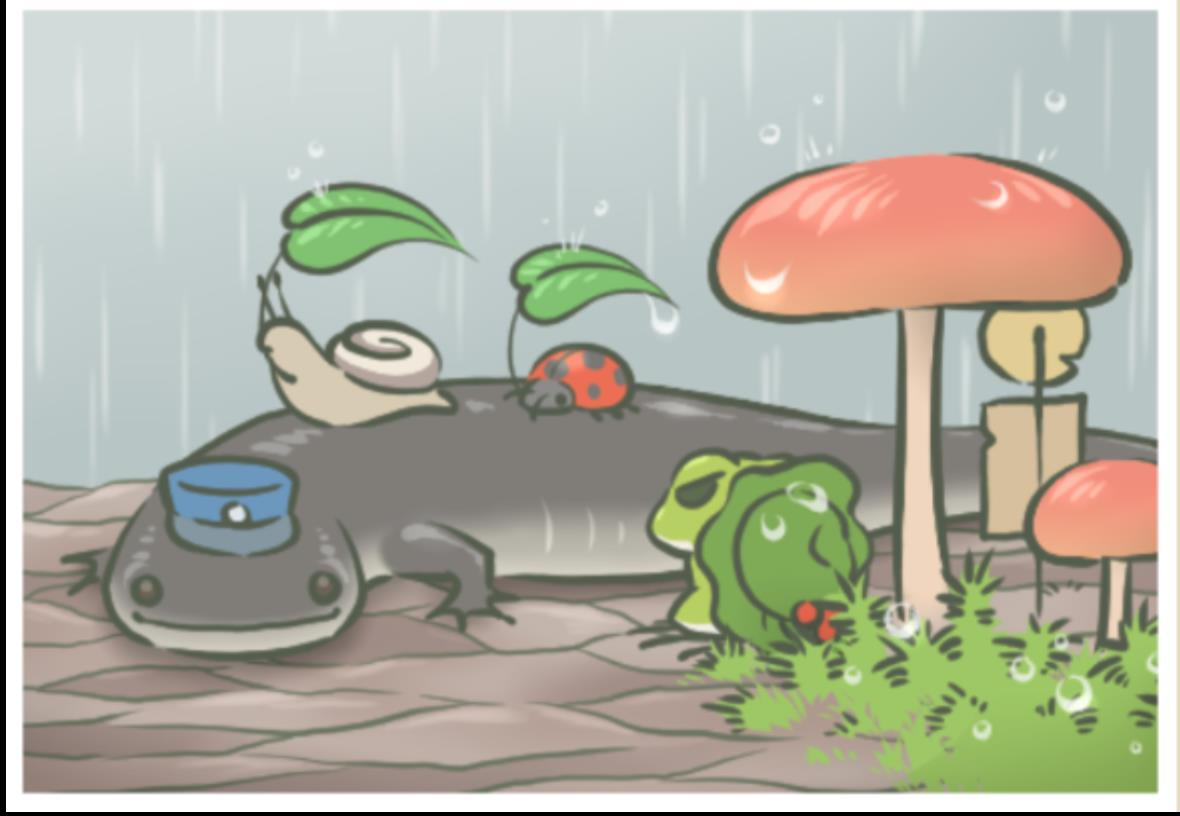
\includegraphics[width=0.7\textwidth]{frog/image/bus.jpg} 
\caption{bus in the forest}
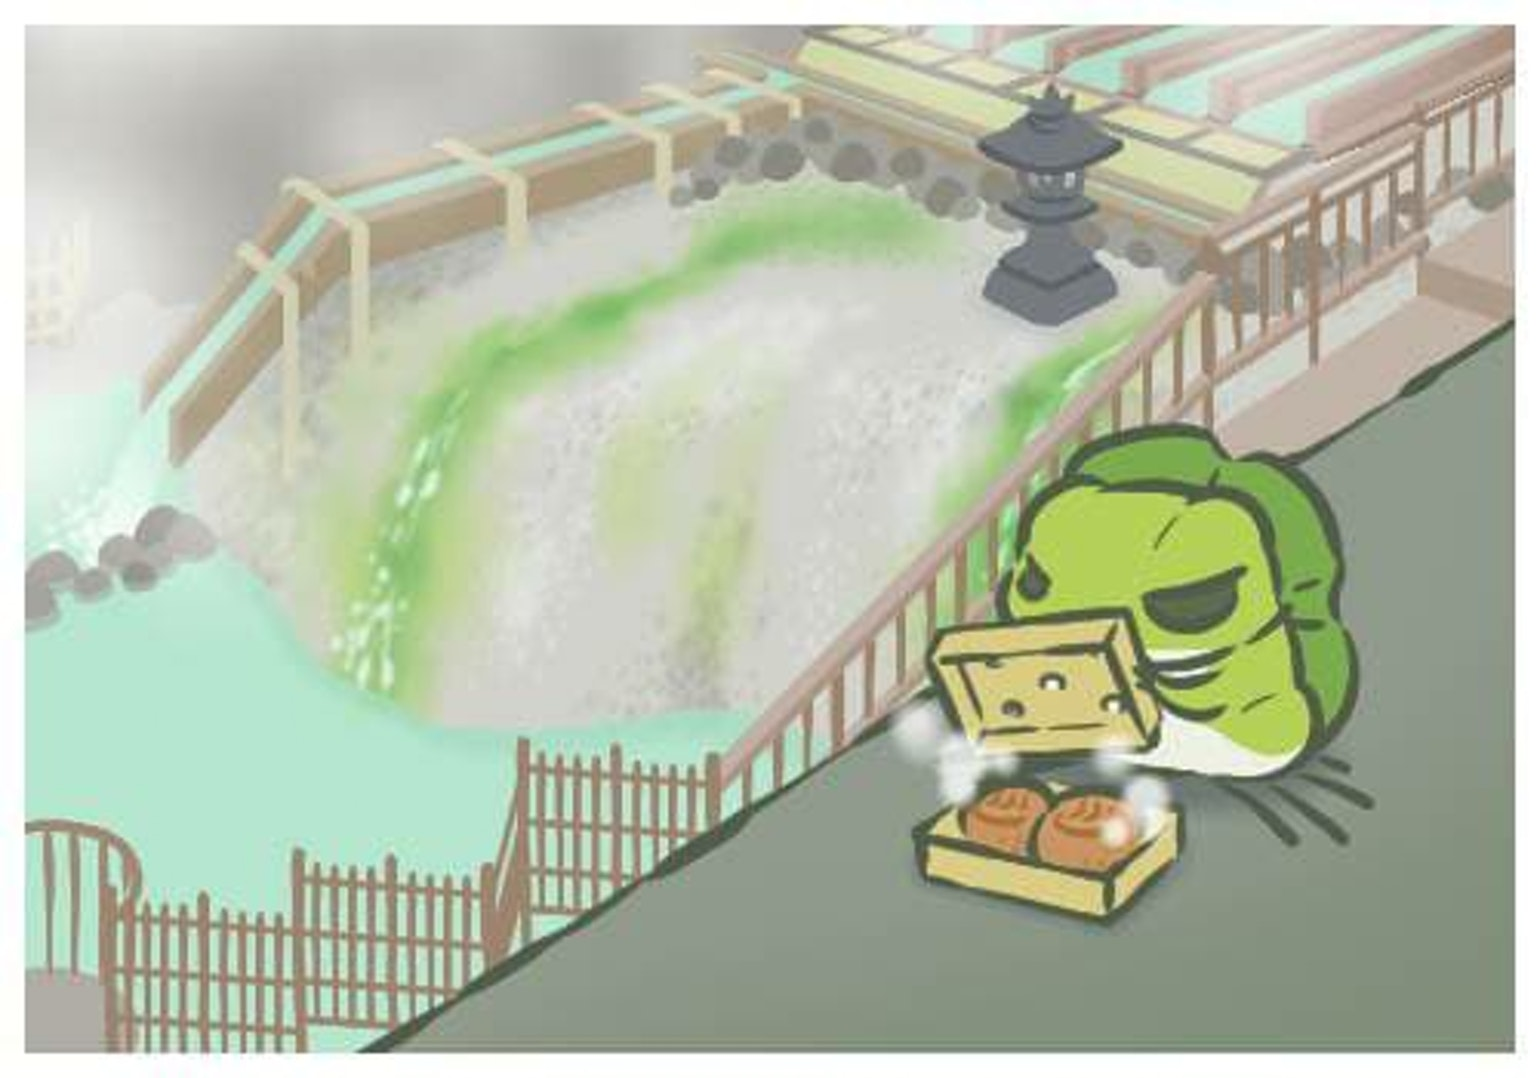
\includegraphics[width=0.7\textwidth]{frog/image/kusatsu.jpg} 
\caption{frog in Kusatsu (Famous japanese sightseeing spot)}
\end{figure}
The game is easy to play, and some players have said it helps them think about parenting and relate to their parents’ anxieties about them. But many players also say they find the game appealing because of its philosophical approach, which teaches that one must learn to surrender control in order to move forward.

Hong Kong blog Refract commented that the game was a reflection of the so-called “Buddhist” attitude adopted by young people, both in Hong Kong and on the mainland. Trapped between an unattainable future and high expectations because of high rent and living costs, they might as well learn to give up their ambitions and live a minimalist life.

“You have to prepare food for the frog, but you have no control over its whereabouts, or how many postcards it will send home. Such kind of uncertainties in interpersonal relationships is very post-modern, and ‘very Wong Kar-wai’,” the blog wrote, in a reference to the Hong Kong filmmaker who meditates on the fluidity and unpredictability of relationships in movies like Chungking Express. “When playing a game where you cannot form strategies to win, you cannot change and escape from that solitude.” 